\section{A Fonte de Alimentação}
\subsection{O Dimensionamento}
A alimentação do \cpr será provida por um cabo de energia. Ele foi dimensionado de forma a suprir a potência elétrica dos equipamentos embarcados no sistema, além de garantir que o robô percorra, sem limitação de distância, toda a extensão da piscina. O \cpr será alimentado por uma tomada perto da piscina, em tensão de $220V$ (padrão Brasília), entretanto, os diversos equipamentos intermos são alimentados em diferentes tensões, fazendo com que seja necessário o uso de uma fonte chaveada para a redução da tensão de alimentação de cada equipamento.

O comprimento do cabo será explicado a seguir. Para o correto dimensionamento de um cabo de energia, de acordo com a literatura, deve-se levar em consideração a distância entre a fonte de energia e a carga, a potência consumida, além da queda de potência do cabo. Assim, o cálculo para a definição da bitola do fio que será utilizado fica determinado pela equação abaixo.

\begin{equation} \label{eq:bitola}
  S = \frac{\sqrt{3} \times IL}{58 \times U}
\end{equation}

Para um fio trifásico de cobre a equação apresenta o cálculo para o seu dimensionamento. Na equação, $S$ é a bitola do fio, em \textsf{mm\textsuperscript{2}}, $I$ é a corrente que passa pelo condutor, em Ampères, $L$ é o comprimento total da fonte de energia até a carga, em metros, $U$ é a queda de tensão suportada pelo fio, em Volts, e 58 é uma constante devido ao material do fio, no caso Cobre.

Para o robô de piscina deste projeto a potência total consumida no robô é de $240W$, assim a corrente que deverá ser suportada no fio é de 1,60 A. Utilizando a equação acima temos que a bitola ideal para o fio será de 6,5 mm\textsuperscript{2}, para o sistema $ca$.

A alimentação dos dois motores das escovas será feito com alimentação em $cc$, assim a Figura \ref{fig:table-wire} apresenta modelo para cálculo da espessura do fio. Para o caso do robô, o fio de alimentação dos motores deverá suportar 1,5 mm\textsuperscript{2}.
\par
\begin{figure}[h]
  \centering
  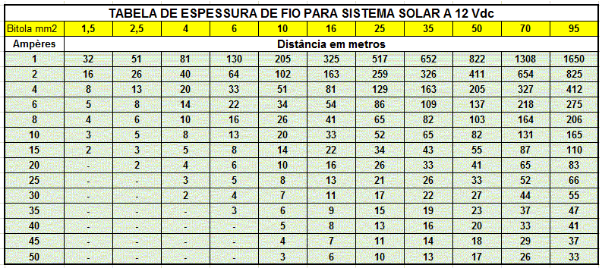
\includegraphics[width=0.9\textwidth]{figures/table-wire.png}
  \caption{Espessura de fio para sistemas solar 12 V em dc.}
  \label{fig:table-wire}
\end{figure}
\FloatBarrier
\par
Como a alimentação interna do robô deve ser feita em duas tensões diferentes, foi escolhido uma fonte chaveada (\textit{Switched-mode power supply}). É uma fonte de alimentação elêtronica que incorpora um regulador chaveado, em outras palavras, um circuito controlador interno que chaveia a corrente, ligando e desligando de forma rápida, mantendo, assim, uma tensão de saída estabilizada. Os parâmetros que serão suficientes para a alimentação do sistema estão explicados a seguir.

Ao contrário das fontes lineares, esse tipo de fonte utiliza-se de circuitos embutidos, fazendo com que este tipo de equipamento seja menor e mais leve, o que seria importante para o produto final, pois traria maior conforto ao cliente. Apresenta uma potência dissipada maior, pois utiliza-se de transistores do tipo FET(\textit{Filed Effect Transistor}), mais vantajoso. Além de dissipar menor quantidade de calor por não apresentar um núcleo de ferro. Esses fatores fazem com que a eficiência desse tipo de equipamento seja melhor.

\subsection{Fonte Chaveada}
Devido a características de baixo volume e peso em comparação a fontes de alimentação convencionais, a fonte de alimentação chaveada é atualmente a mais utilizada em sistemas eletrônico. Importante evidenciar que as fontes chaveadas são sistemas eletrônicos bem mais complexos que as fontes de alimentação convencionais, visto que sua principal vantagem está relacionada à utilização de um interruptor eletrônico durante seu funcionamento[8].

Desse modo a potência elétrica pode ser definida de acordo com a tensão e corrente, sendo essa:
\begin{equation} \label{eq:potencia}
  P = V \times I
\end{equation}

Onde, $P$ é potência em Watts; $V$ é tensão em Volts e $I$ é a corrente em Ampére.

Com isso, quando um transistor está trabalhando na região linear como um controlador de corrente, a potência elétrica do sistema não será nula, gerando assim uma dissipação da potência em forma de calor. Porém, se o transistor estiver operando como um interruptor, a mesma irá gerar uma dissipação de potência bem menor se comparada as demais fontes de alimentação, devido ao processo de chaveamento acontecer em intervalos pequenos [8].

Passando para parâmetros de eficiência, a fonte de alimentação com chaveamento apresenta uma relação de quase 95\% de qualidade em comparação às demais fontes de alimentação sem chaveamento, as quais ficam entorno de 65\%. Além da análise da relação de potência por peso, sendo as fontes convencionais capazes de fornecer 25W/kg e as fontes chaveadas capazes de oferecer 100W/kg [8].

Com base nas informações apresentadas e na possível potência geral do sistema está em torno de 240 Watts, serão utilizadas duas fontes de alimentação chaveada com os seguintes parâmetros elétricos : 110/220 Volts $AC$ para 12 Volts e 10 Ampéres $DC$. Importante ressaltar que o sistema será alimentado por duas fontes independentes ao mesmo tempo, afim de se evitar possíveis danos ao sistema eletrônico devido a corrente de partida dos motores de escovação e da bomba de propulsão.
\par
\begin{figure}[h]
  \centering
  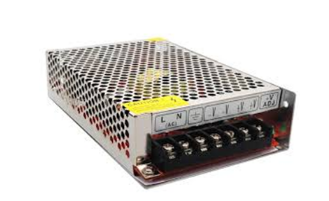
\includegraphics[width=0.6\textwidth]{figures/power-supply.png}
  \caption{Fonte de alimentação Chaveada.}
  \label{fig:power-supply}
\end{figure}
\FloatBarrier
\par
